%%%%%%%%%%%%%%%%%%%%%%%%%%%%%%%%%%%%%%%%%%%%%%%%%%%%%%%%%%%%%%%%%%%%%%
%     File: ExtendedAbstract_sysbase.tex                             %
%     Tex Master: ExtendedAbstract.tex                               %
%                                                                    %
%     Author: Pedro Miranda                                          %
%     Last modified : 29 Dez 2020                                    %
%%%%%%%%%%%%%%%%%%%%%%%%%%%%%%%%%%%%%%%%%%%%%%%%%%%%%%%%%%%%%%%%%%%%%%
% System Baseline Setup.
%%%%%%%%%%%%%%%%%%%%%%%%%%%%%%%%%%%%%%%%%%%%%%%%%%%%%%%%%%%%%%%%%%%%%%
\section{System Baseline}
\label{sec:sys_baseline}

%%%%%%%%%%%%%%%%%%%%%%%%%%%%%%%%%%%%%%%%%%%%%%%%%%%%%%%%%%%%%%%%%%%%%%%%
\subsection{Embedded Software Version}
\label{section:embedded_sw}

%%%%%%%%%%%%%%%%%%%%%%%%%%%%%%%%%%%%%%%%%%%%%%%%%%%%%%%%%%%%%%%%%%%%%%%%
\subsection{IOb-SoC Hardware Platform}
\label{section:iob_soc}

The baseline hardware system used for this work is IOb-SoC~\cite{iob_soc_repo},
an open-source RISC-V SoC platform developed by IObundle.
Figure~\ref{fig:IOb-SoC_complete} presents the block diagram of the system. A
RISC-V soft CPU core controls the system.

\begin{figure}[!htb]
	\centering
	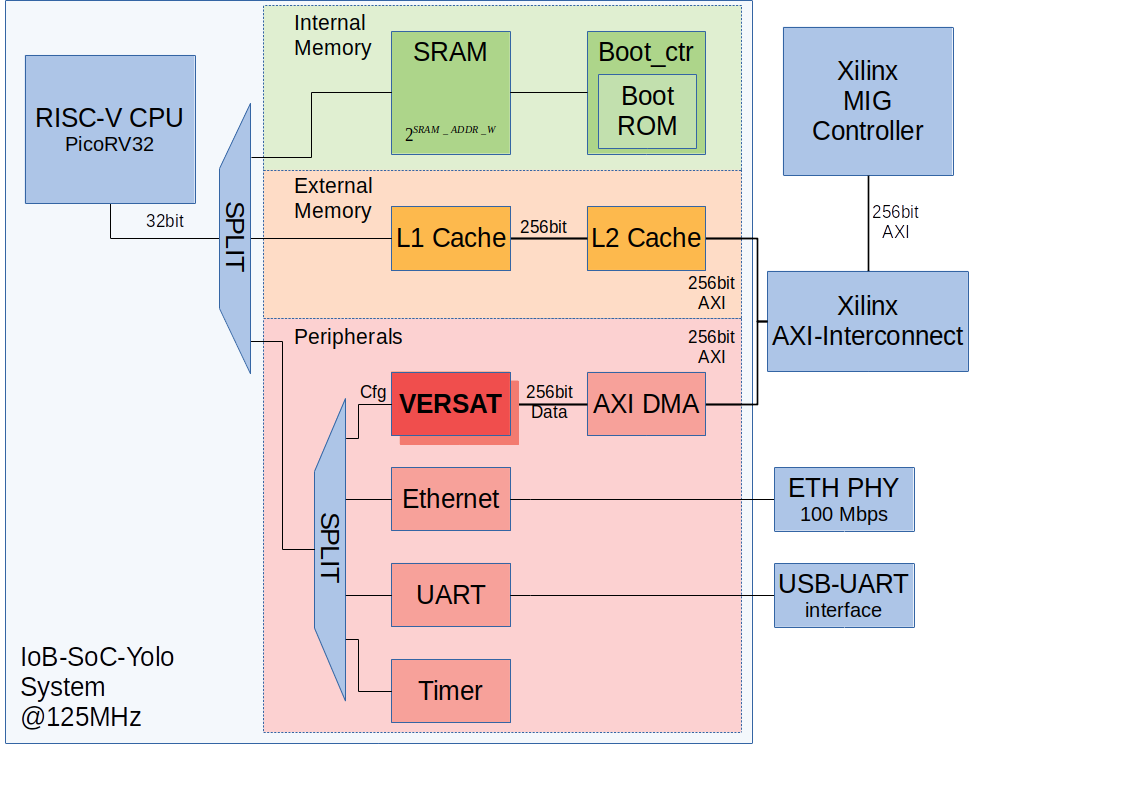
\includegraphics[width=0.6\textwidth]{images/IoB-SoC-Yolo_block_diagram.png}
	\caption{IOb-SoC-Yolo block diagram.}
	\label{fig:IOb-SoC_complete}
\end{figure}

The CPU used is the PicoRV32 RISC-V core~\cite{picorv_repo}, minimally modified
to be integrated into IOb-SoC. The PicoRV32 CPU is designed to use minimal
hardware resources and, as a consequence, has very low performance, taking 4
Cycles Per Instruction (CPI). The CPU can access the internal memory, the
external DDR memory (via cache), and the four peripherals mentioned:
\begin{itemize}
\item the VersatCNN Accelerator Core is the main focus of this work and is used
  to accelerate the convolution operation.
\item the Timer is used to measure performance.
\item the UART is used for programming and basic user runtime messages.
\item the Ethernet module provides a higher bandwidth communication facility
  used to transfer large datasets to IOb-SoC.
\end{itemize}

%%%%%%%%%%%%%%%%%%%%%%%%%%%%%%%%%%%%%%%%%%%%%%%%%%%%%%%%%%%%%%%%%%%%%%%%
